\section{Non-Equilibrium Blunt Body Flows}
Non-Equilibrium flows behind shock waves plays a very vital role in such flow conditions, the chemical composition behind then normal shock in the blunt body resembles the same flow features as the normal shock compositions. Let us assume a streamline that passes through the flow obtained from figure 12.
Let us consider a stagnation streamline that that follows in the blunt body, between a and b, the flow is compressed and slowed, and moves infinitesimally slow to traverse through a and b, because the flow is dissociated and more ionization takes place.

\begin{figure}[ht]
\centering
  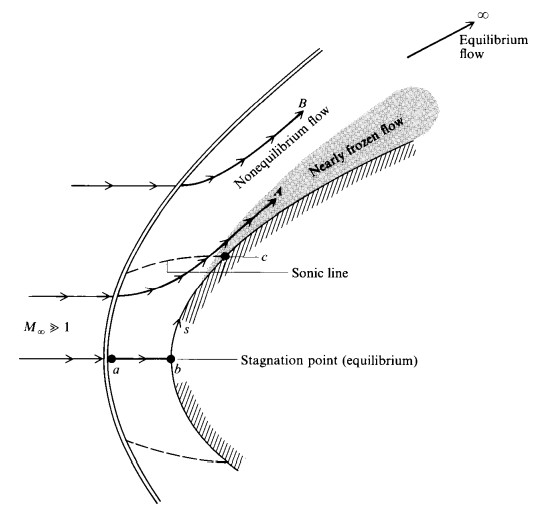
\includegraphics[width=0.7\linewidth]{images/bluntbody_streamline.jpg}
  \caption{Schematic representation of Hypersonic flow around the blunt-body flow field}
  \label{fig:boat1}
\end{figure}

Let us come to the downstream properties where the flow rapidly increases downstream, the surface streamline bc encounters very high changes in temperature and pressure gradients along the flow, Sudden freezing at the surface of the blunt body can be witnessed at the sonic region in the c region of the streamline. After these type of flow features taking place, the body tends to come into equilibrium state after such features, The amount of ionization and dissociation becomes weaker and weaker as we approach the oblique shock region and tends to go to local equilibrium far down stream from the flow.

Similar time marching solution that have been performed for the solution for a simplified gas for simple dissociated gas can be performed using Lax finite difference scheme, later inviscid time marching equilibrium blunt body solution for detailed air chemistry can be obtained. Later explicit MacCormack method was used for shock fitting. The governing equations are as follows,

Equation 1, we see the ci derivatives on the left and spacial derivatives to the right,
\large\[\frac{\partial c_i}{\partial t} = - u \frac{\partial c_i}{\partial x}- v \frac{\partial c_i}{\partial y}- w \frac{\partial c_i}{\partial z} + \frac{ w_i}{\rho}\]
Equation 2 The spacial differences and represented in predictor step in forward difference and backward difference in corrector step
\large\[c_i(t+\Delta t) = c_i(t) + \frac{1}{2}(\frac{\partial c_i}{\partial t}-  \frac{\partial c_i}{\partial y})\Delta t\]
The CFL criterion at the particular time step is given by
\large\[\Delta t {<=}\frac{\Delta x,\Delta x,\Delta z}{1.5[u^2+v^2+w^2]^{1/2}+a}\]
Chemistry time step at the given instant of time is given by
\large \[\Delta t <= 0.1 min|(\frac{\rho c_i}{w_i})|\]

The Delta t is comparatively low in such equations due to its stiff nature in the equations. The processes are very tie consuming to formulate and therefore Li suggested, instead of all these equations, following governing equations at their own time scales and simultaneously adding the general conservation equations that are followed are added into the solving of the governing equations This can considerably lower the actual time steps that are involved in solving the flow physics when compered to the above time method to obtain convergence the flow field. 
In Li method, finite rate equations were assumed, local thermodynamic equilibrium was assumed 
\begin{figure}[ht]
\centering
  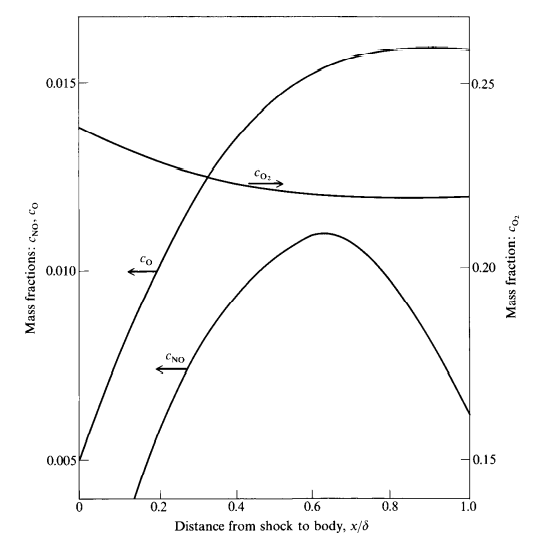
\includegraphics[width=0.5\linewidth]{images/stagnation properties along streamline.png}
  \caption{Mass fractions along the stagnation streamlines along the sphere for free-stream conditions for Li analysis of non equilibrium flow.}
  \label{fig:boat1}
\end{figure}

\begin{figure}[ht]
\centering
  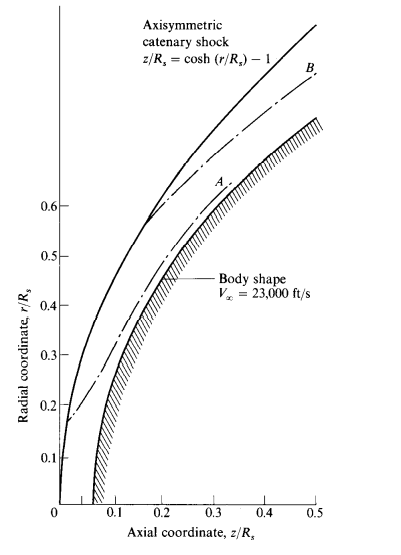
\includegraphics[width=0.3\linewidth]{images/shock_and_blunt.png}
  \caption{Shock and body shapes and calculated streamlines for the non-equilibrium
flow over a blunt body.}
  \label{fig:boat1}
\end{figure}


\begin{figure}[ht]
\centering
  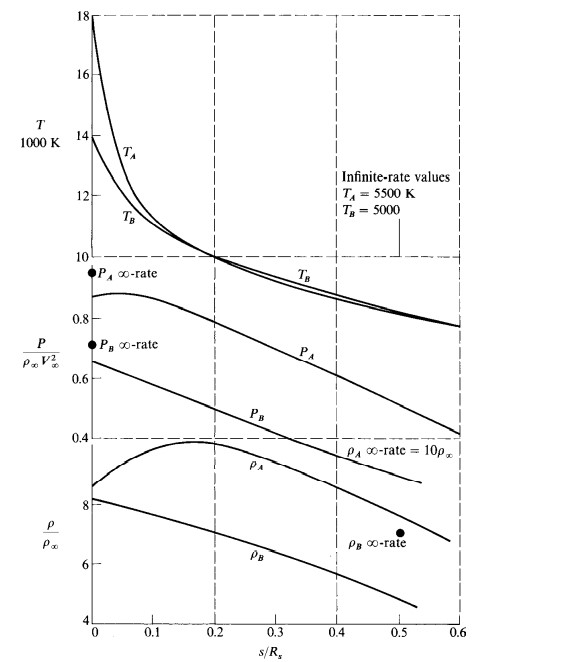
\includegraphics[width=0.4\linewidth]{images/temperature_density_pressure_variation.jpg}
  \caption{Variation of Temperature, Density and Pressure along streamlines A and B in non-equilibrium flow field.}
  \label{fig:boat1}
\end{figure}


The first comprehensive technique was first conducted for non-equilibrium blunt body analysis, the analysis involved was a inverse solution, shape analysis, determination of the shock shape and further finding the body that fits the current shock shape. Hall, replaced the flow field with 7 points with partial derivatives.
The partial differential equations become ordinary differential equation where x derivatives are known numbers, hence this methodology is used to solve by Runge Kutta Method. This is the classical method used to solve non equilibrium flows. In figure 14, variation of flow properties along a and b are given for the given free-stream conditions, the temperature along streamline a shows rapid increases in the temperature and therefore is important in understanding the flow physics and shows the importance of these type of calculations that are involved in the flow. The finite dissipation rate of N2 and O2 plays a major role in the increase of flow temperature. There is gradual increase in pressure and substantial increase in the density of the flow due to non-equilibrium effects. The streamline b passes through a much weaker portion of the shock wave. The relaxation distances are lower when compared to oblique shock wave irrespective of the downstream conditions.
